\documentclass[a4paper,12pt]{book} 

\usepackage{url}
\usepackage{hyperref}
\usepackage{enumerate}
\usepackage{amsmath}
% We're working with A4, which is 21cm by 29.7
\setlength{\paperwidth}{210mm}
\setlength{\paperheight}{297mm}
%\setlength{\hoffset}{-15mm}
\setlength{\voffset}{-25mm}
\setlength{\textheight}{242mm}
\setlength{\topmargin}{10mm}
\setlength{\headheight}{10mm}
\setlength{\headsep}{10mm}
\setlength{\footskip}{1.2cm} %def=30pt=1.054cm

\setlength{\textwidth}{155mm}
\setlength{\oddsidemargin}{5mm}
\setlength{\evensidemargin}{-5mm}

% Espai entre línies de 1.5
\renewcommand{\baselinestretch}{1.5}

\usepackage{fancyhdr}
\pagestyle{fancy}
\pagenumbering{arabic}
% \setlength{\parindent}{0truecm}
\lhead{}
\chead{}
\rhead{}
\lfoot{}
\cfoot{}
\rfoot{}
\renewcommand{\headrulewidth}{0pt}


\everymath{\displaystyle}
\makeindex

\usepackage{titlesec}

\titleformat{\chapter}[block]
  {\normalfont\huge\bfseries\center}{\thechapter.}{1em}{\Huge}
\titlespacing*{\chapter}{-0.5cm}{-1.5cm}{0.5cm}
\renewcommand{\chaptername}{}

\begin{document}



\newlength{\centeroffset}
\setlength{\centeroffset}{-0.5\oddsidemargin}
\addtolength{\centeroffset}{0.5\evensidemargin}
%\addtolength{\textwidth}{-\centeroffset}
\thispagestyle{empty}
\vspace*{\stretch{1}}
\noindent\hspace*{\centeroffset}\begin{minipage}{\textwidth}
% \begin{center}
%       \includegraphics[width=0.8\textwidth]{./../figures/matesLliure.pdf}
% \end{center}
\begin{figure}[H]
\centering
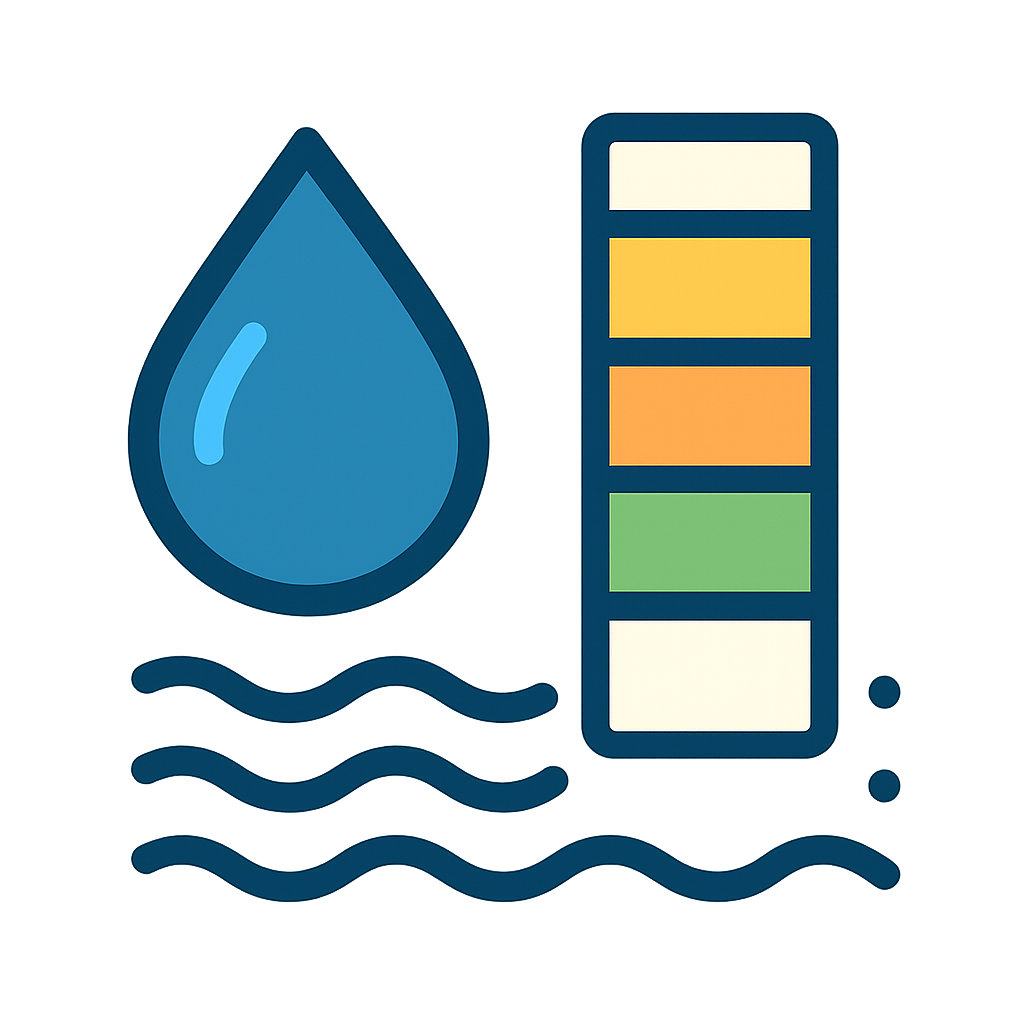
\includegraphics[width=0.45\textwidth]{./Figures/ImatgeTR.png}
\end{figure}
\vspace*{3truecm}

\flushright
{\Huge\bfseries 
  Qualitat de l’aigua:\\
}
\vspace*{0.5truecm}
{\LARGE\bfseries
  Anàlisi comparativa amb tires reactives
}
\noindent\rule[-1ex]{\textwidth}{5pt}\\[4.5ex]
\end{minipage}

\vspace{\stretch{1}}
\noindent\hspace*{\centeroffset}\begin{minipage}{\textwidth}
\flushright
{\bfseries 
	Muhammad Waqas\\
	Tutor: Fernando García Vílchez \\
	Departament de Matemàtiques\\
	Institut Sants\\
}
\end{minipage}
%\addtolength{\textwidth}{\centeroffset}
\vspace{\stretch{2}}


\pagebreak

\vspace*{16truecm}

	\begin{quote}
	\textbf{Avís legal}

	  Copyright \copyright{}  Muhammad Waqas.
	  Es garanteix permís per copiar, distribuir i modificar aquest document segons els termes de la GNU Free Documentation License, versió 1.3 o qualsevol posterior publicada per la Free Software Foundation. Es disposa d'una còpia d'aquesta llicència a~\href{http://www.fsf.org}{http://www.fsf.org} i a l'annex~\ref{a:license}.
	\end{quote}	





\endinput


\frontmatter

\cleardoublepage

\chapter{Agraiments}


\cleardoublepage
\setcounter{tocdepth}{2}
\renewcommand\contentsname{Índex de continguts}
\tableofcontents
\label{i:tableofcontents}

\mainmatter
\pagestyle{fancy}
\fancyhf{}
\fancyhead[RE,LO]{Institut Sants}
\fancyhead[LE,RO]{\leftmark}
\fancyfoot[RE,LO]{Institut Sants}
\fancyfoot[LE,RO]{\thepage}
\renewcommand{\headrulewidth}{2pt}
\renewcommand{\footrulewidth}{1pt}

\chapter{Introducció}

L’aigua és un recurs fonamental per a la vida. Cada dia la fem servir per beure, cuinar, netejar o regar, i sovint donem per fet que sempre serà accessible i segura. Tanmateix, la seva qualitat no és un aspecte trivial: segons dades de l’Organització Mundial de la Salut \cite{OrgaMS}, més de 2.000 milions de persones al món consumeixen aigua contaminada, la qual cosa pot provocar greus problemes de salut i afectar els ecosistemes aquàtics.

Aquest treball de recerca (TR) es dividirà en 3 \textbf{capítols essencials}:

\begin{itemize}
  \item En el \textbf{Capítol 4}~\nameref{c:Metodologia}, em centraré en explicar les eines que he utilitzat per poder completar correctament aquest treball, així com les raons del seu ús.

  \item El \textbf{Capítol 3}~\nameref{c:RecercaPrevia} es centra en l’estudi de diversos paràmetres físics, químics i biològics que permeten determinar la qualitat de l’aigua. A través d’aquests indicadors (com el pH, la duresa, la presència de nitrats, el clor, la temperatura o la presència de microorganismes) és possible entendre millor fins a quin punt l’aigua és apta per al consum humà i per al manteniment dels ecosistemes.

  \item Finalment, en el \textbf{Capítol 5}~\nameref{c:Partpra}, desenvoluparé la part pràctica, on realitzaré un total de tres experiments amb tota la informació obtinguda de la recerca prèvia, per poder calcular la qualitat de l’aigua. Els resultats d’aquests experiments seran recollits i analitzats a les conclusions del treball. (\textbf{PON REFERENCIAS})
\end{itemize}

\textbf{EN ÀNGLES / IN ENGLISH}






\chapter{Objectius}

L'objectiu principal del meu treball és fer recerca en el camp de la Química. Tot i les limitacions que tenim en recursos materials i humans (el meu tutor és professor de Matemàtiques), hem creat un grup de recerca tan real com ha estat possible.

En aquest grup de recerca el meu tutor ha actuat com el cap de recerca i ha fixat una sèrie de requisits propis del grup de treball. En canvi, jo he actuat com a investigador fixant el tema, fent la formació prèvia, ...
A continuació detallarem els requisits fixats per cadascuna de les parts:

\subsubsection*{Requisits del grup de recerca}


\subsubsection*{Requisits de l'investigador}


%%%%% Aprofita el que tens per completar el que falta i si falta alguna cosa ho afegeixes.
%%%%%%%%%%%%%%%%%%%%%%%%%%%%%%%%%%%%%%%%%%%%%%%%%%%%%%%%%%%%%%%%%%%%%%%%%%
En aquest treball, l’objectiu principal és analitzar la qualitat de l’aigua mitjançant l’ús de tires reactives. Per a fer-ho de manera adequada, ha estat necessari dur a terme una recerca prèvia sobre els paràmetres de qualitat de l’aigua, els valors mínims i màxims recomanats i alguns dels molts components químics i biològics que poden estar-hi presents. Aquesta fase teòrica ha permès adquirir una base sòlida per a la experimentació.

A més, aquest treball no es limita a la recerca bibliogràfica i l’anàlisi de resultats, sinó que també ha implicat un procés d’aprenentatge personal. He hagut d’adaptar-me a l’ús de noves eines experimentals, proporcionades pel meu tutor de TR, Fernando García, i aprendre a aplicar-les correctament. Aquest procés metodològic es descriu amb més detall al capítol de Metodologia (vegeu capítol~\nameref{c:Metodologia}).

Com a objectiu personal, vull que aquest treball no només tingui un interès acadèmic, sinó que també sigui capaç de resultar interesant per a persones que habitualment no s’interessen per temes científics. Fer entenedor un tema tècnic com la qualitat de l’aigua és un repte personal que vull aconseguir.

Finalment, el treball de recerca també té un objectiu formatiu: aprendre a cercar informació de manera autònoma, a estructurar un treball científic i a realitzar una experimentació pròpia. Tot aquest procés em proporciona experiència i em prepara per a futurs reptes acadèmics i professionals.


% \chapter{Objectius}
% vull aprendre
%
% \chapter{Introducció}

L’aigua és un recurs fonamental per a la vida. Cada dia la fem servir per beure, cuinar, netejar o regar, i sovint donem per fet que sempre serà accessible i segura. Tanmateix, la seva qualitat no és un aspecte trivial: segons dades de l’Organització Mundial de la Salut \cite{OrgaMS}, més de 2.000 milions de persones al món consumeixen aigua contaminada, la qual cosa pot provocar greus problemes de salut i afectar els ecosistemes aquàtics.

Aquest treball de recerca (TR) es dividirà en 3 \textbf{capítols essencials}:

\begin{itemize}
  \item En el \textbf{Capítol 4}~\nameref{c:Metodologia}, em centraré en explicar les eines que he utilitzat per poder completar correctament aquest treball, així com les raons del seu ús.

  \item El \textbf{Capítol 3}~\nameref{c:RecercaPrevia} es centra en l’estudi de diversos paràmetres físics, químics i biològics que permeten determinar la qualitat de l’aigua. A través d’aquests indicadors (com el pH, la duresa, la presència de nitrats, el clor, la temperatura o la presència de microorganismes) és possible entendre millor fins a quin punt l’aigua és apta per al consum humà i per al manteniment dels ecosistemes.

  \item Finalment, en el \textbf{Capítol 5}~\nameref{c:Partpra}, desenvoluparé la part pràctica, on realitzaré un total de tres experiments amb tota la informació obtinguda de la recerca prèvia, per poder calcular la qualitat de l’aigua. Els resultats d’aquests experiments seran recollits i analitzats a les conclusions del treball. (\textbf{PON REFERENCIAS})
\end{itemize}

\textbf{EN ÀNGLES / IN ENGLISH}



%
% \chapter{Objectius}

L'objectiu principal del meu treball és fer recerca en el camp de la Química. Tot i les limitacions que tenim en recursos materials i humans (el meu tutor és professor de Matemàtiques), hem creat un grup de recerca tan real com ha estat possible.

En aquest grup de recerca el meu tutor ha actuat com el cap de recerca i ha fixat una sèrie de requisits propis del grup de treball. En canvi, jo he actuat com a investigador fixant el tema, fent la formació prèvia, ...
A continuació detallarem els requisits fixats per cadascuna de les parts:

\subsubsection*{Requisits del grup de recerca}


\subsubsection*{Requisits de l'investigador}


%%%%% Aprofita el que tens per completar el que falta i si falta alguna cosa ho afegeixes.
%%%%%%%%%%%%%%%%%%%%%%%%%%%%%%%%%%%%%%%%%%%%%%%%%%%%%%%%%%%%%%%%%%%%%%%%%%
En aquest treball, l’objectiu principal és analitzar la qualitat de l’aigua mitjançant l’ús de tires reactives. Per a fer-ho de manera adequada, ha estat necessari dur a terme una recerca prèvia sobre els paràmetres de qualitat de l’aigua, els valors mínims i màxims recomanats i alguns dels molts components químics i biològics que poden estar-hi presents. Aquesta fase teòrica ha permès adquirir una base sòlida per a la experimentació.

A més, aquest treball no es limita a la recerca bibliogràfica i l’anàlisi de resultats, sinó que també ha implicat un procés d’aprenentatge personal. He hagut d’adaptar-me a l’ús de noves eines experimentals, proporcionades pel meu tutor de TR, Fernando García, i aprendre a aplicar-les correctament. Aquest procés metodològic es descriu amb més detall al capítol de Metodologia (vegeu capítol~\nameref{c:Metodologia}).

Com a objectiu personal, vull que aquest treball no només tingui un interès acadèmic, sinó que també sigui capaç de resultar interesant per a persones que habitualment no s’interessen per temes científics. Fer entenedor un tema tècnic com la qualitat de l’aigua és un repte personal que vull aconseguir.

Finalment, el treball de recerca també té un objectiu formatiu: aprendre a cercar informació de manera autònoma, a estructurar un treball científic i a realitzar una experimentació pròpia. Tot aquest procés em proporciona experiència i em prepara per a futurs reptes acadèmics i professionals.



\chapter{Recerca prèvia}
\label{c:RecercaPrevia}
\section{Què és la qualitat de l’aigua?}
% La qualitat de l'aigua es un terme que es refereix a les caracteristicas fisicas, quimicas y bilogicas de l'aigua. Per determinar-la, s'analitzan alguns paràmetres.

Segons la Wikipedia~\cite{WikiAgua}, s'entén la qualitat de l'aigua com les `característiques químiques, físiques, biològiques i radiològiques de l'aigua`, en relació amb necessitats humanes.

La Fundació Aquae~\cite{Fundacionaquae} indica que la qualitat de l'aigua és un conjunt de paràmetres, com temperatura, contingut mineral i bacteris, mesurats i comparats amb estàndards, per definir si l'aigua és apta per a fins determinats o no.

En aquest TR analitzarem diversos paràmetres per analitzar la qualitat de l'aigua que es classifiquen en tres grups:
\begin{enumerate}
  \item \textbf{Paràmetres químics}: són els relacionats amb la composició química de l’aigua; indiquen si és potable o contaminada. En concret, estudiarem el pH, la duresa, els nitrats i els nitrits, el clor i els metalls pesants. Els paràmetres químics seran explicats a la secció~\ref{sec:pq}.
  \item \textbf{Paràmetres físics}: mesuren característiques visibles o mesurables sense canviar la composició de l’aigua. Els paràmetres físics seran explicats a la secció~\ref{sec:pf}. En aquesta secció, estudiarem la importància de la temperatura, el color, l’olor i el sabor en la qualitat de l’aigua.
  \item \textbf{Paràmetres biològics}: indiquen la presència de microorganismes que poden ser patògens. Els paràmetres biològics seran explicats a la secció~\ref{sec:pb}. En aquesta secció, explorarem els coliformes fecals, els protozous presents en l’aigua i els bioindicadors.
\end{enumerate}


\section{Paràmetres químics} \label{sec:pq}

\subsection{Què és el pH i per què és important?}
El pH és una mesura que serveix per establir el nivell d’acidesa o alcalinitat d'una dissolució. La `p` ve de `potencial` i l'`H` ve de l’àtom d’hidrogen, per això el pH és el potencial de l’hidrogen. \textbf{Fonts}: \cite{PH}

S'expressa com el logaritme negatiu de base 10 de la concentració de ions d'hidrogen: $ \text{pH} = -\log_{10} [\mathrm{H}^+] $.

A la fórmula la ${H}^+$ és la concentració de ions d'hidrogen en la solució, mesurat en mols per litre (mol/L). $-\log_{10}$ és el logaritme en base 10, el signe negatiu s'utilitza amb l'objectiu que el pH sigui un número positiu. La raó és perquè el logaritme d'un número menor que 1 és negatiu.

D'altra part, el \textbf{pOH} és una mesura de concentració de ions hidroxil ${OH}^-$ en una dissolució. S'expressa com el logaritme negatiu de base 10 de la concentració de ions hidroxil, i a diferència del pH, s'utilitza per mesurar el nivell d’alcalinitat d'una dissolució. Es calcula amb la formula  $ \text{pOH} = -\log_{10} [\mathrm{OH}^-] $.
\subsubsection{ Quina relació hi ha entre el nivell d'acidesa i el pH?}
Les dissolucions àcides tenen una alta quantitat de ions d'hidrogen. Això significa que tenen baixos valors de pH, i per tant, el seu nivell d'acidesa és elevat. Així que una dissolució serà més o menys àcida depenent de la quantitat d'hidrogen que contingui aquesta. \textbf{Fonts}: \cite{PH}

D'altra banda, les dissolucions bàsiques (alcalines) tenen baixes quantitats de ions d'hidrogen. Això vol dir que tenen alts valors de pH, i per tant el seu nivell d'acidesa és baix.
\subsubsection{Escala del pH}
\begin{figure}[h!]
\centering
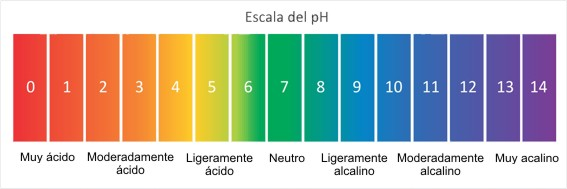
\includegraphics[width=0.9\textwidth]{./Figures/EscaladepH.png}
\caption{Escala del pH}
\label{fig:escaladeph}
\end{figure}
L'escala de pH s'utilitza per mesurar el grau d'acidesa d'una dissolució, i com que el pH està relacionat amb el pOH, coneixent el grau d'acidesa d'una dissolució, també podem saber el seu grau d'alcalinitat (basicitat). \textbf{Fonts}: \cite{PH}

Com podem observar a la figura \ref{fig:escaladeph}, el valor del pH va del 0 al 14. Les substàncies amb pH igual a 0 són més àcides; les que tenen el pH = 7 són neutres, i les que tenen pH = 14 són les menys àcides, per tant, són les més bàsiques. \textbf{Fonts i Fonts d'imatge}: \cite{PH}

\subsubsection{Què ens diu el pH sobre la qualitat de l'aigua?}
El pH és un paràmetre fonamental entre els paràmetres; com he dit abans, indica el grau d'acidesa o alcalinitat. El pH depèn de la quantitat d'hidrogen que conté l'aigua.

Un pH d'1 ens diu que la substància és molt àcida i, per tant, perillosa. L'àcid clorhídric (HCl(aq)) té aproximadament aquest pH. A l'altre extrem de l'escala, amb un pH aproximat de 14, tenim sosa càustica (NaOH). Gràcies a l'escala de pH (figura \ref{fig:escaladeph}), podem saber si la dissolució és més àcida o bàsica. En general, un pH de 7, és a dir, neutre, seria el més òptim en la majoria dels casos; és un pH similar al del nostre cos, la suor, etc. \textbf{Fonts}: \cite{PH}
\subsubsection{Instrument de mesura}
El \textbf{pH-metre} és un instrument utilitzat per mesurar el pH d’una dissolució. Va ser construït per \textbf{Arnold Orville Beckman} l’any \textit{1934}.
\begin{figure}[H]
\centering
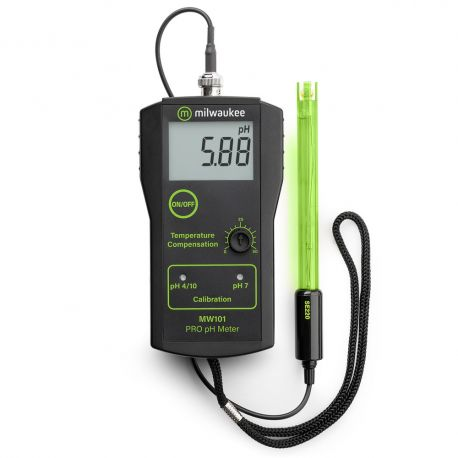
\includegraphics[width=0.3\textwidth]{./Figures/pHmetre.png}
\caption{Imatge del pH-metre actual}
\label{fig:pH-metre}
\end{figure}
El model de Beckman era més gran que el model actual del pH-metre
\begin{figure}[H]
\centering
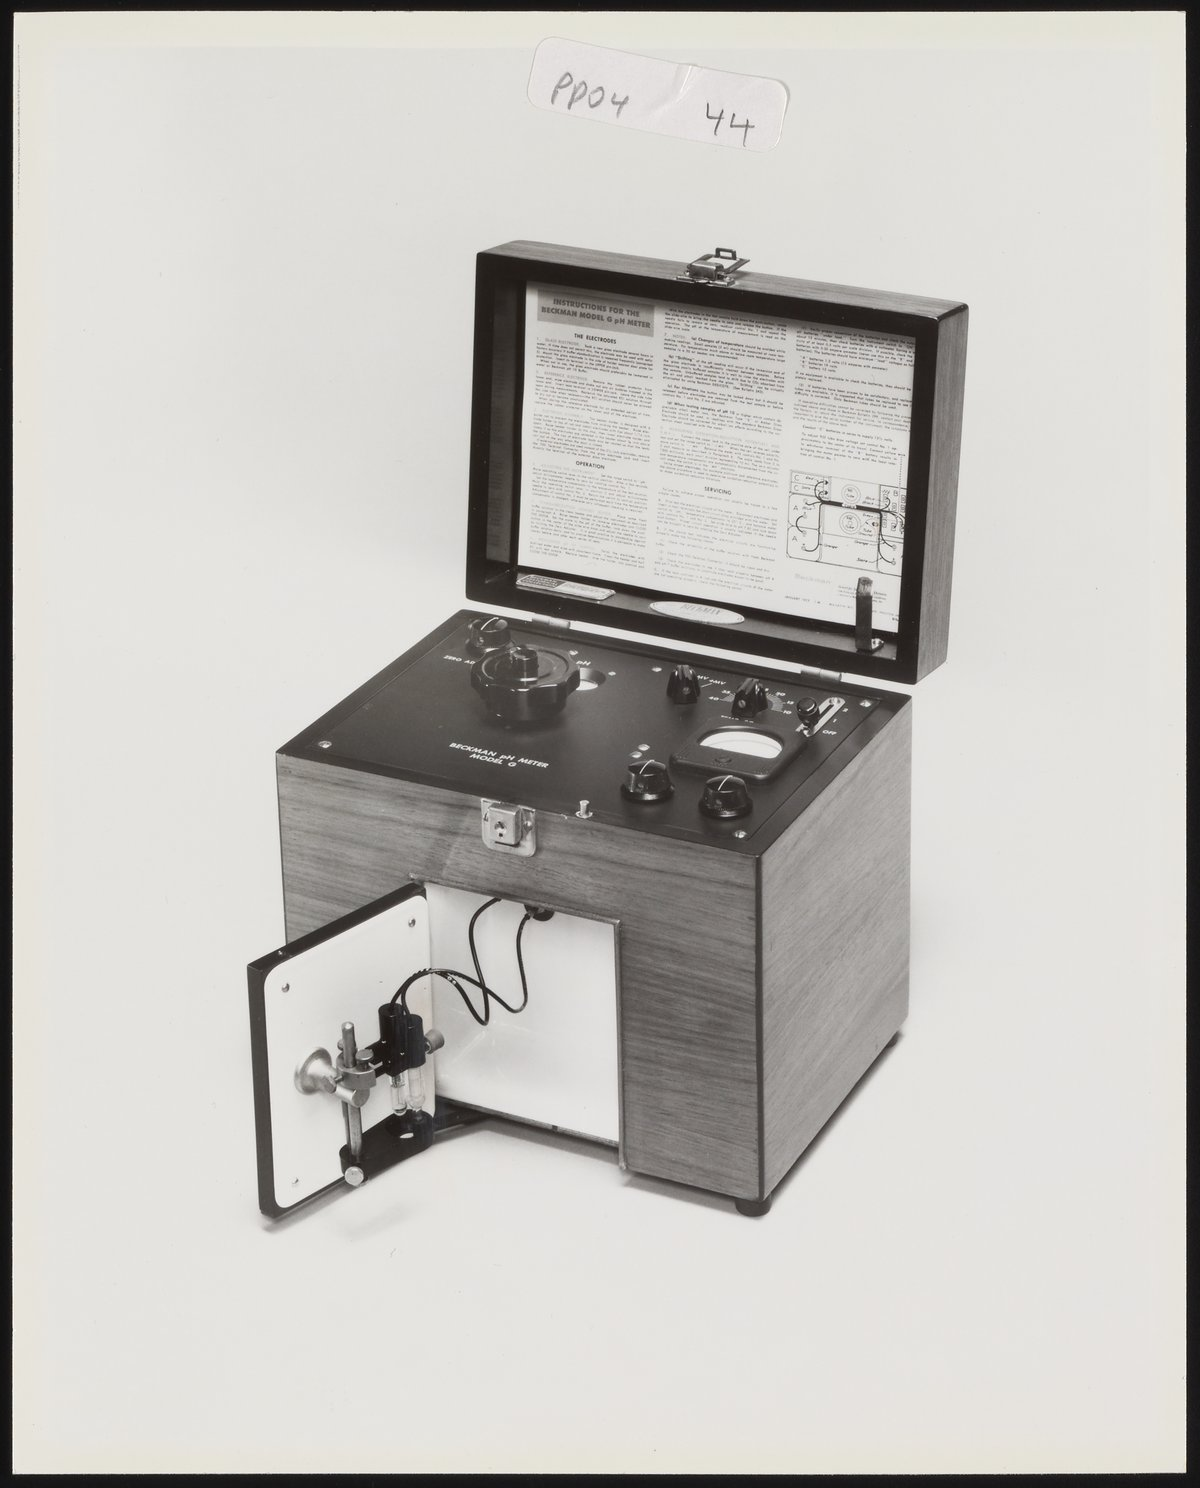
\includegraphics[width=0.3\textwidth]{./Figures/modelbeckman.png}
\caption{Imatge del pH-metre (model de Beckamn)}
\label{fig:pH-metre}
\end{figure}

\subsection{Què és la duresa de l’aigua i com ens afecta?} \label{subsec:duresa}
Es la concentració de compostos minerals en una certa quantitat d'aigua, especialment sals de magnesi i calci.\\
L'aigua `dura` te una alta concentració d'aquestes sals i l'aigua `suau`, te una concentració baixa d'aquestes. La duresa es pot calcular amb la següent formula: (mg/L de Calci (Ca) + mg/L de Magnesi (Mg) x 4.2 )/10 \textbf{Fonts}: \cite{Fasca}

% \textit{Fonts:} \cite{Fasca}\\

% \subsubsection{Què ens diu la OMS?}
\textbf{Què ens diu la OMS?} L'Organització Mundial~\cite{OrgaMS} de la Salut no considera que la duresa de l'aigua tingui un impacte negatiu en l'organisme. En una guia, afirma que els paràmetres per al consum oscil·len entre 100 i 300 mg/l de carbonat de calci, encara que el llindar de tolerància pot estar per sobre o per sota en funció de la normativa de cada país.

En general, la concentració desitjable es considera inferior a 100 mg/l (aigua de més qualitat) i que per sobre de 500 mg/l qualitat ja no és acceptable. En el cas concret d'Espanya, la normativa tecnològica-sanitària estableix un valor de contingut de calci de fins a 100 mg/l amb un límit màxim de tolerància de 200 mg/l.


% % \subsubsection{Instrument de mesura}
% Per mesurar la duresa podem utilitzar els \textbf{test kits de duresa}.
% Es un conjunt d’eines i reactius que s’utilitzen per determinar la quantitat de calci i magnesi.
% Amb aquestes dades i fent servir la fórmula; (mg/L de Calci (Ca) + mg/L de Magnesi (Mg) x 4.2 )/10, poden determinar el nivell de duresa de una dissolució.
% \begin{figure}[H]
% \centering
% 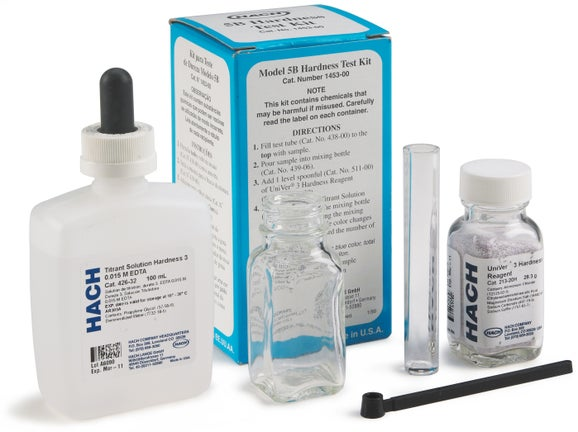
\includegraphics[width=0.3\textwidth]{./Figures/testduresa.png}
% \caption{Imatge del kit de duresa}
% \label{fig:kitsduresa}
% \end{figure}
%
% \textit{Fonts:} \cite{Fasca}


\subsection{Què són els nitrats i nitrits i per què ens han de preocupar?} \label{subsec:nitratsnitrits}
El nitrat \(\mathrm{NO_3^-}\) és un compost químic format bàsicament per nitrogen i oxigen. Naturalment es troba en el sòl i l'aigua, per la qual cosa és un nutrient fonamental per a molts éssers vius.

Quan paguem la terra per millorar el seu rendiment, utilitzem productes de nitrogen, ja siguin fertilitzants minerals o orgànics com els fems. A aquest augment de nitrats, hem d'afegir el plus que representa nitrogen contingut en aigua de reg (aigua utilitzada per el reg de conreus o jardins). Per tant, el nivell final d'aquest compost pot ser alt en moltes ocasions.

Amb el temps, i essencialment a causa de l'acció d'alguns bacteris, aquests nitrats evolucionen en nitrits \(\mathrm{NO_2^-}\), ions considerats més tòxics.
\subsubsection{El nitrit i les seves conseqüències}
El nitrit s'origina en les fruites profundes que es produeixen quan el sistema de reg mou el nitrat al sòl. Aquest risc és més alt quan s'utilitza el reg de la superfície. La contaminació de l'aigua superficial pot tenir conseqüències tan greus com la mort de la fauna aquàtica a llarg termini.

Com hem vist, l'excés de nitrit pot causar la seva contaminació a l'aigua, però també als cultius que estan regats amb aquesta aigua contaminada. Per tant, moltes verdures es poden veure afectades.

Aquestes grans quantitats de nitrits a l'aigua poden tenir un impacte negatiu en la salut de les persones. Per evitar problemes, l'OMS recomana un límit de 50 mil·ligrams de nitrat per litre. \textbf{Fonts:} \cite{Scielo}; en aquest treball es menciona la recomanació de l'OMS sobre el nitrat.

% \subsubsection{Instrument de mesura}
% Per mesurar el nitrat i el nitrit podem utilitzar un \textbf{kit de prova de nitrat-nitrit}, que són mètodes per mesurar aquests elements amb més precisió.
% \begin{figure}[H]
% \centering
% 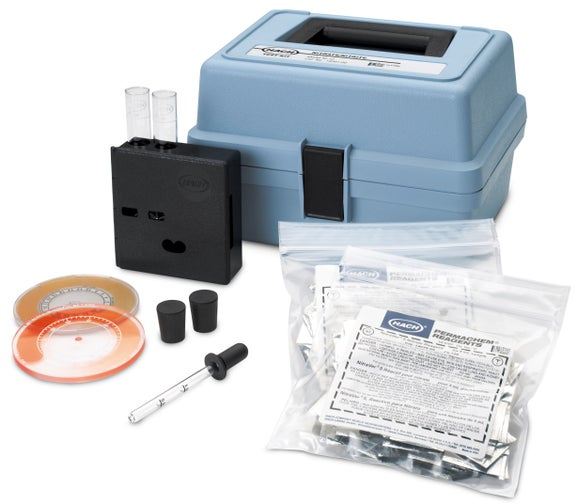
\includegraphics[width=0.3\textwidth]{./Figures/nitratnitrit.png}
% \caption{Imatge de kit de prova de nitrat-nitrit}
% \label{fig:kitnitrats}
% \end{figure}

\subsection{Clor: per què és essencial en l’aigua que bevem?} \label{subsec:clor}
El clor és un element químic, un gas groc verdós, dens i amb una olor irritant. S'utilitza principalment per desinfectar l'aigua, eliminant així les bacteris i altres microorganismes nocius.

La seva presència és considerada l'últim pas per a la potabilització de l'aigua. Desinfecta microorganismes patògens que causen malalties als humans; per aquesta raó, la seva desinfecció és fonamental en la protecció de la salut pública.

Tot i que existeixen altres mètodes de desinfecció, el clor ha sigut el responsable de l'augment de l'esperança de vida a l'Europa del passat segle XX. Però, anteriorment, fa cinc segles, s'utilitzaven altres formes de desinfecció més rudimentàries, com bullir l'aigua.

La revista Rain of life \cite{RoF} classifica la cloració (procés de desinfecció que utilitza clor) com “probablement el més significatiu progrés de la salut pública del mil·lenni” l'any 1997.

Per tant, el clor és un producte químic amb l'objectiu de desinfectar l'aigua. Tanmateix, l'ús d'aquest component químic \textbf{no és segur.}
\subsubsection{Com el clor de l'aigua potable afecta la salut}
Segons el doctor en Medicina Josep Lluís Berdonces, qui es basa en diferents estudis sobre aquest tema, la cloració de l’aigua pot tenir efectes nocius sobre la salut de les persones. Té en la seva composició àcids húmics i fúlvics. Les conseqüències d’aquests components químics sobre la salut humana són variades. Molts d’ells tenen una gran afinitat per unir-se amb els diversos greixos del cos. \textbf{Fonts:} \cite{RoF}
% \subsubsection{Instrument de mesura}
% Per mesurar el clor, podem utilitzar un \textbf{fotòmetre portàtil de clor}.
% \begin{figure}[H]
% \centering
% 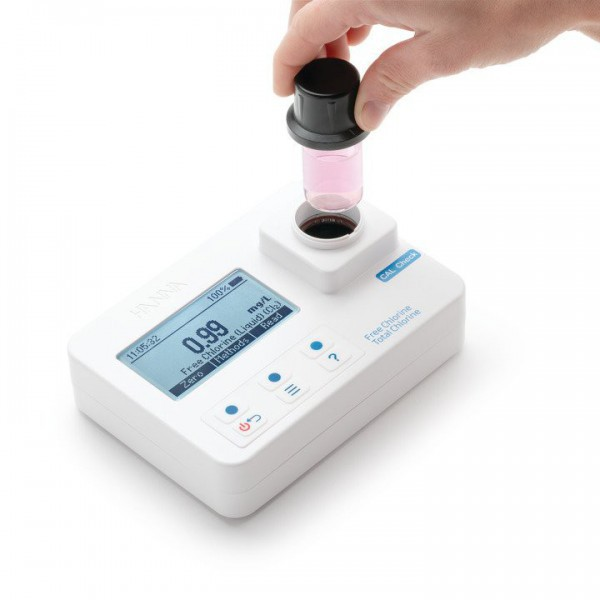
\includegraphics[width=0.3\textwidth]{./Figures/Cloro.jpg}
% \caption{Imatge del fotòmetre portàtil de clor}
% \label{fig:clormetre}
% \end{figure}

\subsection{Presència i efectes dels metalls pesants en l’aigua potable} \label{subsec:metallspesats}
El terme de `metalls pesants` es refereix a qualsevol element químic metàl·lic que té una alta densitat i pot ser tòxic o verinós a baixes concentracions.

Alguns metalls pesants com el coure ($Cu$), el seleni ($Se$), i el zinc ($Zn$) són essencials per mantenir el metabolisme del cos humà. No obstant això, en altes quantitats poden conduir a l'enverinament. Aquesta intoxicació pot ocórrer si es consumeix aigua amb algun d’aquests metalls.
\subsubsection{Com es contamina l’aigua amb metalls pesants?}
El principal motiu és la contaminació industrial. Una altra font de contaminació pot ser els abocaments d'aigües residuals. Hi ha casos en què l’aigua pateix un procés d’enriquiment de metalls pesants, ja que passa per roques que contenen aquests metalls en la seva composició.
\subsubsection{Alguns metalls pesants presents a l'aigua}
\begin{enumerate}
 \item \textit{\textbf{Alumini}}
 Tot i que l'alumini no és un metall pesat, representa aproximadament el 8 per cent de la superfície terrestre i és el tercer element més abundant. Està disponible per a la ingestió humana a través de l'aigua potable.
 \item \textit{\textbf{Arsènic}}
 L'arsènic és la causa més freqüent d'enverinament per metalls pesants aguts en adults. L'arsènic també es pot trobar en el subministrament d'aigua, el que porta a l'exposició en marisc, bacallà, haddock i alguns altres aliments marins
 \item \textit{\textbf{Coure}}
 El coure a altes concentracions pot ser tòxic. Els efectes per a la salut són els següents: pot causar vòmits, diarrea, pèrdua de força o, per a l'exposició severa, la cirrosi del fetge.
 \item \textit{\textbf{Ferro}}
 El ferro és un metall pesant comú a l'aigua, s'ha de tenir cura de menjar suplements de ferro, i en la dieta pot enverinar agudament els nens petits. La ingestió representa la major intoxicació per ferro per a les persones.
 \item \textit{\textbf{Mercuri}}
 El mercuri es genera naturalment en el medi ambient en la desgasificació de l'escorça terrestre i les emissions volcàniques.
\end{enumerate}
\textbf{Fonts:~\cite{WikiMetales},~\cite{carbotecnia}}
% \subsubsection{Instrument de mesura}
% Per mesurar els metalls pesants (no tots) podem utilitzar un \textbf{kit d’anàlisi de metalls pesants}, que encara que aquests kits no proporcionin un valor exacte, podem aproximar-lo i així mesurar els nostres metalls pesants.
% \begin{figure}[H]
% \centering
% 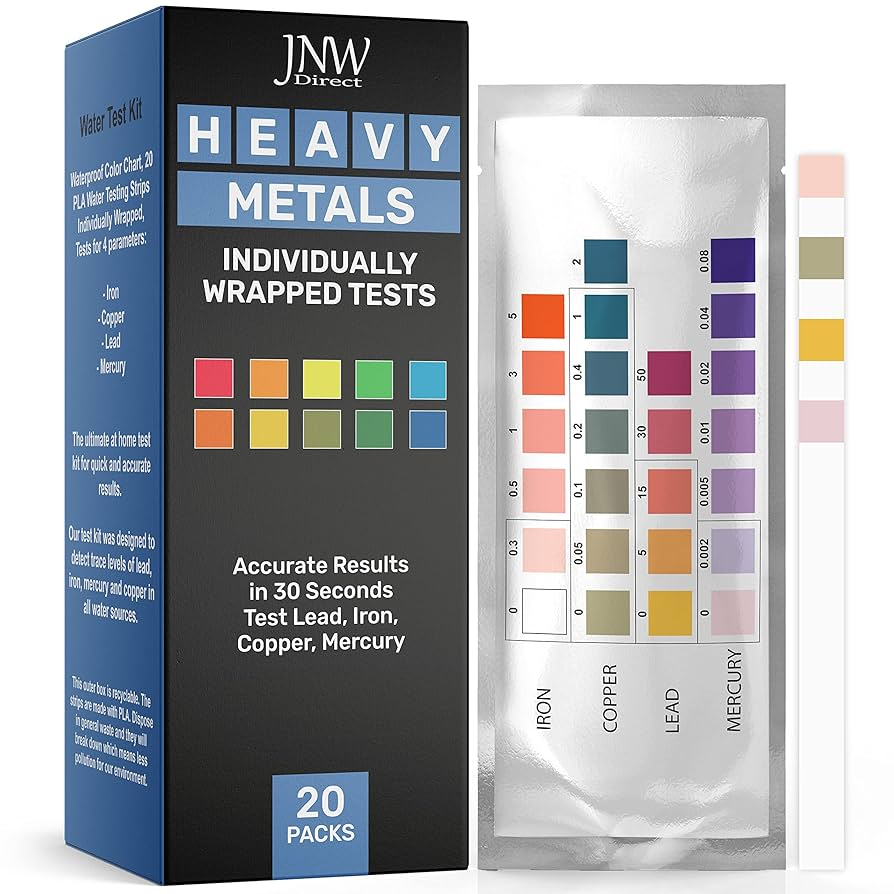
\includegraphics[width=0.3\textwidth]{./Figures/metales.jpg}
% \caption{Imatge de kit d’anàlisi de metalls pesants}
% \label{fig:kitmetall}
% \end{figure}
\section{Paràmetres físics} \label{sec:pf}

\subsection{Temperatura de l’aigua: què ens diu sobre la vida aquàtica?} \label{subsec:temperatura}
La temperatura és un paràmetre físic que permet mesurar les sensacions de calor o fred. En termes científics, és una mesura de l’energia cinètica de les molècules que el componen, és a dir, com de molt es mouen o s’agiten aquestes molècules.
\subsubsection{Quina relació te amb la qualitat de l'aigua?}
Un gran exemple de la importància de la temperatura és a la vida aquàtica. Per exemple, l’aigua freda reté més oxigen; això fa que sigui vital per als peixos i altres éssers aquàtics. Quan aquesta temperatura augmenta, la quantitat d’oxigen disminueix, afectant així la supervivència d’aquests organismes.

També afecta el metabolisme dels organismes: els animals aquàtics i les plantes tenen un rang de temperatura ideal. Si aquest rang és superat per molt de temps, els organismes poden patir malalties o fins i tot aquest canvi pot portar-los a la mort.

Una dada curiosa és que, a temperatures més altes, algunes substàncies tòxiques es tornen més actives o més perilloses per als organismes.\\
\textit{Fonts:} \cite{UCM}

\subsection{Color de l’aigua: què ens indica sobre la seva qualitat?} \label{subsec:color}
És un dels paràmetres \textbf{organolèptics} (organolèptics són les característiques d'un producte que es pot percebre amb els sentits, en aquest cas, la vista) que indica la qualitat de l'aigua per al consum humà. Està relacionat amb les substàncies dissoltes o les \textbf{partícules en suspensió} (són partícules sòlides o líquides molt petites disperses en l’aire).
\subsubsection{La seva importància amb la qualitat de l'aigua}
El color és important perquè pot alertar sobre la presència de substàncies que, en combinar-se amb desinfectants com el clor (més informació sobre el clor al apartat~\ref{subsec:clor}), poden generar \textbf{subproductes nocius}.

`Els compostos com ferro, manganès o coure, i especialment les substàncies húmiques (àcids fúlvics i húmics), són els principals responsables del color. Tot i que aquestes substàncies són inofensives per si soles, poden formar compostos tòxics durant la desinfecció amb clor.` (Higiene Ambiental, 2019, \textit{Color del agua, parámetro indicador de calidad}\\
 \textit{Fonts:} \cite{HA}

\subsection{Què ens diu l’olor i el sabor de l’aigua?} \label{subsec:olorisabor}
L’olor i el sabor són, com el color, \textbf{paràmetres organolèptics} essencials en l’avaluació de la qualitat de l’aigua. La presència d’olors i sabors inusuals pot indicar possibles problemes de contaminació o alteració biològica, i s’hauria de considerar una alerta sanitària, fins i tot si l’aigua compleix amb els altres paràmetres químics i biològics.

\section{Paràmetres biològics} \label{sec:pb}
\subsection{Coliformes fecals: què ens diuen sobre l’aigua que bevem?} \label{subsec:coliformes}
Els coliformes fecals són bacteris coliformes que estan presents a l’intestí dels animals de sang calenta (humans, gossos, vaques, ànecs, etc.). Aquests bacteris surten del cos a través dels excrements.

La raó per la qual són tan importants en l’aigua és perquè, si es detecten coliformes fecals, això indica que hi ha una contaminació amb matèria fecal i, per tant, hi ha un major risc de presència d’altres microorganismes perillosos, com virus o paràsits.
\subsubsection{Malalties que poden causar els bacteris coliformes}
\begin{enumerate}
 \item \textit{\textbf{Gastrointestinals}} que causen diarrea i vòmits.
 \item \textit{\textbf{La disenteria}}, és una afecció inflamatòria de l’intestí, especialment del còlon, que produeix diarrea greu amb moc o sang als excrements.
 \item \textit{\textbf{Virus}}, que poden causar hepatitis.
\end{enumerate}
\textbf{En conclusió}, la presència de bacteris coliformes pot indicar la presència d'altres patògens més perillosos, com E. coli (és un tipus de bacteri que pot produir malalties i causar diarrea).
\subsection{Protozous a l’aigua} \label{subsec:protozous}
A l’aigua es poden trobar microorganismes com els protozous, alguns d’aquests poden ser patògens i poden causar malalties gastrointestinals si s’ingereixen. Alguns exemples d’aquests protozous són el Giardia, Cryptosporidium, Entamoeba histolytica i Toxoplasma gondii. Però la majoria dels protozous no representen un risc per a la salut humana, i es troben comunament en ambients aquàtics.
\subsection{Bioindicadors} \label{subsec:indicadorbiologic}
Un indicador biològic o \textbf{bioindicador} de l’aigua són organismes vius que poden utilitzar-se per avaluar la qualitat de l’aigua. Aquests organismes poden proporcionar informació sobre la presència de contaminants o l’estat general de l’ecosistema aquàtic.

Una vegada explicat què vol dir qualitat de l’aigua i alguns dels paràmetres més importants, donaré una mica més de context i la importància global de la qualitat de l’aigua.

\section{OMS (Organització Mundial de la Salut)}
És un organisme especialitzat de les Nacions Unides que es dedica a la salut a nivell mundial. El seu objectiu principal és que totes les persones assoleixin el màxim grau de salut possible.
\subsection{Estàndards de la qualitat de l’aigua de l’OMS}
Des de 1958, la OMS (Organització Mundial de la Salut) va establir uns estàndards per a la qualitat de l’\textbf{aigua potable} que serveixen com a referència \textbf{internacional} per garantir la seguretat i potabilitat de l’aigua.
\subsubsection{Què són realment els estàndards per a l’aigua potable?}
Són regulacions establertes per la legislació interna dels països per controlar el nivell de contaminants a l’aigua de consum humà en cada nació.

Els estàndards nacionals se centren en l’establiment de límits per regular els contaminants que presenten un gran risc d’afectar la salut pública, i aquests es basen en la seva factibilitat segons els recursos econòmics i ambientals disponibles per a cada país.

Per establir aquests estàndards, la OMS va haver de realitzar una investigació i una anàlisi que els permetessin verificar si aquests estàndards complirien la seva missió principal: protegir la salut pública. La OMS s’encarrega únicament de concentrar i establir les pautes, les quals són adaptables pels països. Els països poden escollir lliurement si establir aquestes normes o no, ja que el país també té dret d’establir les seves pròpies normes, les quals poden ser menors, iguals i/o més estrictes que les recomanades per la OMS.
\subsubsection{Estàndards establerts per l’OMS}
\textbf{Coliformes fecals:} La quantitat de coliformes fecals recomanada per les guies de l’OMS és de 0 UFC (unitats formadores de colònies) / 100 ml.\\

\textbf{Arsènic:} L’estàndard establert per l’OMS per a l’arsènic a l’aigua és de 0,01 mg/L.\\

\textbf{Cadmi}: És un dels metalls més tòxics i és biopersistent. El nivell establert per l’OMS és de 0,003 mg/L, el qual és adoptat pel 38,88 per cent dels països. \\

\textbf{Cianur:} És una substància química potencialment letal que actua com a tòxic mitjançant la inhibició de certes proteïnes. Les quantitats de cianur permeses als països presenten una alta variabilitat. El valor recomanat per l'OMS es de 0,07 mg/L.\\

\textbf{Coure:}  El coure és un metall important perquè posseeix propietats que el fan extraordinàriament útil per a una diversitat d’usos. El nivell recomanat de coure per l’OMS és de 2 mg/L, el qual és adoptat pel 26,31 per cent dels països.\\

\textbf{Crom:} És un metall que es troba espontàniament a l’aigua, al sòl i a les roques. Les guies de l’OMS estableixen un nivell màxim recomanable de 0,05 mg/L.\\

\textbf{Mercuri:} Metall que ocorre de forma natural en l’ambient i que té diverses formes químiques. El nivell establert per l’OMS és de 0,001 mg/L.\\

\textbf{Nitrat:} Entre un rang de 10 mg/L i un màxim de 50 mg/L. Això permet inferir que el nivell de nitrats està ben administrat per les legislacions nacionals de cadascun dels països, els quals es mantenen dins dels estàndards de l’OMS.\\

\textbf{Nitrit:} L’estàndard establert per l’OMS és de 3 mg/L.\\

\textbf{Plom:} És un metall tòxic i molt perillós per a la salut. El plom entra a l’aigua potable primordialment com a resultat de la corrosió o desgast dels materials que estan al sistema de subministrament d’aigua. La concentració de plom recomanada per l’OMS és de 0,01 mg/L.\\

\textbf{Seleni:} És un micromineral antioxidant que prevé les reaccions excessives d’oxidació. L’OMS va establir un nivell de 0,01 mg/L.\\

\textbf{Alumini:} La recomanació de l’OMS és permetre com a màxim 0,2 mg/L perquè no cause cap dany a la salut humana.\\

\textbf{Amoníac:} És un gas incolor reconegut per molta gent, ja que s’utilitza en sals aromàtiques. L’OMS estableix una concentració màxima de 1,5 mg/L.\\

\textbf{Clorur:} El clorur és una sal composta per dos elements, un dels quals és el clor. Totes les sals de clorur són molt solubles en aigua. La concentració màxima recomanada per l’OMS és de 250 mg/L.\\

\textbf{Ferro:} És un dels minerals més abundants de l’escorça terrestre. És molt freqüent en les aigües subterrànies. L’OMS recomana 0,3 mg/L.\\

\textbf{Sodi:} És un metall tou, reactiu i de punt de fusió baix. Com que el sodi és explosiu i tòxic a l’aigua, l’OMS recomana un nivell màxim de concentració de 200 mg/L.\\

\textbf{Zinc:} L’OMS recomana una concentració màxima de 3 mg/L.\\

\textbf{Color:} Les guies de l’OMS recomanen un límit màxim de 15 UCV (unitats de color veritable).\\

\textit{Fonts:} \cite{Estan}

\subsection{Impacte global en la salut publica}
Es important mencionar l'impacte en la salut publica, com la mala qualitat de l'aigua afecta la salut globalment.
\subsubsection{Informació general}
L'aigua segura i fàcilment accessible és important per a la salut pública, ja sigui utilitzada per beure, per a ús domèstic, per produir aliments o amb finalitats recreatives. La millora de l'oferta, el \textbf{sanejament} (el sanejament és l’eliminació segura d’aigües residuals i deixalles.) i la gestió dels recursos hídrics poden impulsar el creixement econòmic dels països i contribuir en gran mesura a la reducció de la pobresa.
% \\ \textit{Fonts:} \cite{OrgaMS}

El 2010, l'Assemblea General de les Nacions Unides va reconèixer explícitament el dret humà al subministrament d'aigua i al sanejament. Totes les persones tenen dret a una disponibilitat contínua de quantitats suficients d'aigua segura, físicament accessible, assequible i d'una qualitat acceptable per a ús personal i domèstic.\\
\textit{Fonts:} \cite{OrgaMS}

\subsubsection{Aigua i salut}
L’aigua contaminada contribueix a la transmissió de malalties.
%com les anteriorment mencionades.
Si no es gestiona de forma apropiada, la població queda exposada a riscos per a la salut que, en realitat, es poden prevenir. \textbf{Fonts:} \cite{OMS2}

La mala gestió de les aigües residuals provoca que milions de persones consumeixin aigua amb contaminació biològica i química, incloent-hi arsènic, fluorurs i plom. \textbf{Fonts:} \cite{OMS2}

Segons l’OMS, cada any al voltant d’un milió de persones moren a causa de malalties diarreiques relacionades amb l’aigua insalubre, el sanejament deficient o la mala higiene de mans, provocant així unes 395 000 morts de nens menors de cinc anys. Hi ha malalties, com l’esquistosomiasi, que es transmeten pel contacte amb aigua infestada. \textbf{Fonts:} \cite{OMS2}
En definitiva, garantir l’accés a aigua potable segura no només és una necessitat bàsica, sinó també una de les mesures de salut pública més eficaces per prevenir malalties i salvar vides. \textbf{Fonts:} \cite{OMS2}

\subsection{Accions de l’OMS per garantir aigua segura i salut pública}
L’OMS treballa arreu del món per evitar malalties causades per l’aigua contaminada i ajudar els governs a fixar normes i objectius que protegeixin la salut. Publica recomanacions sobre la qualitat de l’aigua per beure, reutilitzar aigües residuals de forma segura i per activitats recreatives, amb un enfocament basat en prevenir riscos. \textbf{Fonts:} \cite{OMS2}

Des del 2004, les seves \textit{Guies de qualitat de l’aigua de consum humà} expliquen com establir objectius de salut, fer plans per garantir que l’aigua sigui segura des que es capta fins que arriba a la llar, i fer controls independents per comprovar que tot funciona bé. L’OMS dona suport als països amb materials pràctics, ajuda directa, lleis adaptades a cada lloc i reforç de la vigilància. \textbf{Fonts:} \cite{OMS2}

Des del 2014, revisa productes per tractar aigua a casa, assegurant que eliminin microbis perillosos i ajudant els països a usar-los correctament. \textbf{Fonts:} \cite{OMS2}

També treballa amb \textbf{UNICEF} (Fons de les Nacions Unides per a la Infància (\textit{United Nations International Children's Emergency Fund})) per millorar l’aigua, el sanejament i la higiene als centres de salut. El 2015 van crear l’eina \textbf{WASH FIT} perquè centres petits, sobretot en països amb pocs recursos, puguin revisar els seus serveis, detectar problemes i aplicar millores concretes. Un informe del 2023 dona idees pràctiques per aconseguir aigua segura, sanejament i higiene en aquests centres. \textbf{Fonts:} \cite{OMS2}

\subsection{WASH FIT}
És una guia pràctica de l’Organització Mundial de la Salut (OMS) i UNICEF per millorar la qualitat de l’atenció sanitària en establiments de salut de països amb ingressos baixos i mitjans. Es centra en l’aigua, el sanejament, la higiene i la gestió de residus, utilitzant un enfocament de gestió de riscos per identificar, avaluar i abordar problemes relacionats amb aquests aspectes.\textbf{Fonts:} \cite{Wash1},~\cite{Wash2}

% \subsubsection{Països on s'ha utilitzat aquesta guia}
WASH FIT s’ha utilitzat en més de 40 països de tots els continents:
% . Països com: \\
Benín, Bhutan, Burundi, Burkina Faso, Cambodja, Txad, Comores, República Democràtica del Congo, Equador, Etiòpia, Filipines, Ghana, Guatemala, Guinea, Guinea Bissau, Haití, Índia, Indonèsia, l’Iraq, Kenya, Libèria, Madagascar, Malawi, Maldives, Mali, Mauritània, Moçambic, Myanmar, Nepal, Nicaragua, Níger, Perú, República Democràtica Popular Lao, Ruanda, Sierra Leone, Sudan del Sud, Tanzània, Tadjikistan, Togo, Uganda, Veneçuela, Vietnam, Zàmbia i Zimbabwe. \\
\textbf{Fonts:} \cite{Wash1},~\cite{Wash2}

% Aquí dono per finalitzada la meva part de RecercaPrevia, la veritat és que he après molts conceptes i moltes coses que no sabia sobre la qualitat de l’aigua i alguns elements químics i biològics. A continuació, començaré la meva part pràctica, uns \textbf{3 experiments} que duré a casa per intentar, com bé he dit abans, mesurar la qualitat de l’aigua.


\input{./capitols/Marc Pràctic/Marc Pràctic}

\chapter{Metodologia}
Per explicar la part de metodologia, hauré d'explicar molta informació relacionada amb la informàtica, i intentaré explicar-ho tot de manera que es pugui entendre. Després d’aquesta explicació informàtica, procediré a explicar els materials que utilitzo en els experiments de la part pràctica d’aquest treball.
\vspace{0.3truecm}

Per explicar la part de metodologia, hauré d’explicar molta informació relacionada amb la informàtica, i intentaré explicar-ho tot de manera que es pugui entendre. Després d’aquesta explicació informàtica, procediré a explicar els materials que utilitzo en els experiments de la part pràctica d’aquest treball.\\

Explicaré la informació de manera clara; el primer punt que explicaré és sobre les màquines virtuals.

\section{Màquina virtual}
\subsection{Què és una màquina virtual (VM)?}
Una màquina virtual és un entorn informàtic que funciona com un sistema aïllat amb la seva pròpia CPU (Unitat Central de Processament), memòria, interfície de xarxa i emmagatzematge, el qual es crea a partir del hardware.

\textit{\textbf{Hardware:}} Són tots els components físics d’un sistema informàtic, és a dir, les parts tangibles que es poden veure i tocar.

Les màquines virtuals utilitzen sotware en un ordinador físic (host) per replicar o emular la funcionalitat d’un ordinador diferent. En resum, una màquina virtual és un ordinador simulat dins d’un ordinador real.

Les màquines virtuals funcionen igual que els ordinadors normals: tenen un sistema operatiu, emmagatzemen fitxers, executen programes, etc.

\subsection{Tipus de màquines virtuals}
Les VM poden tenir diferents tasques en funció del tipus de màquina virtual utilitzada.
\begin{enumerate}
 \item \textbf{Màquina virtual de procés}: Serveix per executar un programa com si fos natiu, sense importar el sistema operatiu o el hardware real. No instal·la un sistema operatiu complet, sinó que permet executar programes d’una altra plataforma.

 \textbf{Avantatges:}
 \begin{enumerate}[1)]
  \item Consumeix pocs recursos (RAM i CPU) comparat amb un sistema operatiu complet.
  \item Pots executar programes en qualsevol sistema operatiu compatible.
  \item Si falla, no afecta el sistema operatiu principal.
 \end{enumerate}
 \textbf{Desavantatges:}
 \begin{enumerate}[1)]
  \item Només funciona per a un tipus de programa o plataforma específica (ex. Java).
  \item No pots executar un sistema operatiu complet, només aplicacions.
  \item Accés limitat al sotware: no pot utilitzar tot el potencial del PC.
 \end{enumerate}

 \item \textbf{Màquina virtual de sistema}: Serveix per emular un sistema operatiu complet dins d’un altre; per exemple, pots tenir Linux dins de Windows, o Windows dins de Linux.

  \textbf{Avantatges:}
 \begin{enumerate}[1)]
  \item Permet executar un sistema operatiu complet dins d’un altre.
  \item Pots provar diferents sistemes operatius sense tocar el PC real.
  \item Cada màquina virtual està aïllada, així que errors o virus no afecten el sistema principal.
 \end{enumerate}
 \textbf{Desavantatges:}
 \begin{enumerate}[1)]
  \item Consumeix molts recursos: necessita RAM, CPU i espai al disc.
  \item Pot ser més lenta que usar un sistema operatiu natiu.
  \item Configurar i mantenir diverses màquines virtuals pot ser més complex.
 \end{enumerate}
\end{enumerate}

\subsection{Quina he utilitzat jo?}
Jo no he utilitzat cap maquina virtual, l'eina que he utilitzada és un \textbf{sistema operatiu}.

\section{Sistema operatiu}
\subsection{Què és un sistema operatiu i quina difèrencia hi ha amb la maquina virtual?}
\subsection{Avantatges i Desavantatges}
\subsection{Quin sistema operatiu he utilizat per el treball?}
\section{Xubuntu}
Per aquest treball he utilitzat el sistema operatiu \textit{Xubuntu}\cite{xubuntu}.
\subsection{Què és Xubuntu?}
L’\textbf{Ubuntu} és un sistema operatiu basat en \textit{Linux} (la informació sobre Linux està explicada en una altra secció).

Abans d’explicar més sobre Xubuntu, hem de fer la següent pregunta: què és un sistema operatiu? \\

Un sistema operatiu (SO) és un programa o un conjunt de programes que actua com a intermediari entre el hardware d’un ordinador i les aplicacions que utilitzem, permetent que aquestes s’executin i gestionant els recursos del sistema. (\textit{\textbf{Font:}} \href{https://desarrollarinclusion.cilsa.org/tecnologia-inclusiva/que-es-un-sistema-operativo/#:~:text=Un\%20sistema\%20operativo\%20es\%20un,placa\%20de\%20red\%2C\%20entre\%20otros.}{Desarrollar Inclusión}) \\

Continuant amb l’explicació de Xubuntu: Xubuntu és un SO gratuït que va ser llançat a l’octubre de 2004 per Canonical. Està basat en Linux i deriva de Debian (vegeu informació de Debian). Ubuntu és de codi obert, cosa que significa que tant el sistema com les seves aplicacions estan disponibles per ser estudiades sense cap cost.

\subsection{Per a què serveix Xubuntu?}
Hi ha una infinitat de propòsits, però els que més destaquen són els que descriuré a continuació:
\begin{enumerate}
 \item \textbf{Navegar per internet:} Inclou navegadors com Firefox, optimitzat.
 \item \textbf{Programar i desenvolupar software:} És molt utilitzat per desenvolupadors gràcies a la seva compatibilitat amb una infinitat d’eines de desenvolupament.
 \item \textbf{Utilitzar aplicacions d’oficina:} LibreOffice, Thunderbird o GIMP estan disponibles i són fàcils d’instal·lar.
 \item \textbf{Servidors web i bases de dades:} Ubuntu és la distribució de Linux més popular per a hosting i servidors al núvol.
 \item \textbf{Educació i tasques acadèmiques:} Moltes institucions i escoles l’empren per la seva gratuïtat.
 \item \textbf{Substituir Windows en ordinadors antics:} Consumeix pocs recursos comparat amb el SO de Microsoft, cosa que permet prolongar la vida útil del hardware.
\end{enumerate}

\textit{\textbf{Fonts:}} \href{https://www.godaddy.com/resources/es/crearweb/que-es-ubuntu-y-para-que-sirve}{Equipo de Contenidos de GoDaddy}

\subsection{Per què vaig escollir Xubuntu?}
La principal raó és perquè Ubuntu és gratuït i de codi obert; això fa que sigui accessible per a tothom. Té una gran comunitat, cosa que fa que sigui fàcil trobar ajuda i, per últim, perquè és fàcil d’utilitzar per a principiants.







    \chapter{Resultats}



\chapter{Conclusions}
\label{c:conclusions}

% Aquest treball de recerca m'ha permès abordar l'estudi de la qualitat de l’aigua des de diverses perspectives: teòrica, pràctica i personal. A nivell científic, hem pogut identificar i comprendre els principals paràmetres que defineixen la qualitat de l’aigua, aprendre a mesurar-los amb eines senzilles com les tires reactives i interpretar els resultats obtinguts amb rigor.
%
% La part pràctica m'ha posat a prova els coneixements previs i les habilitats adquirides, permetent-me experimentar de manera controlada i analitzar les dades obtingudes. Els experiments han evidenciat la importància de seguir correctament els procediments per obtenir mesures fiables i han generat recomanacions útils per a futurs treballs similars.
%
% A més, aquest projecte ha tingut un gran valor formatiu. He après a cercar informació de manera autònoma, a utilitzar eines professionals de recerca i documentació com Linux, GitHub i LaTeX, i a organitzar el treball de manera eficient. Tot això ha contribuït al desenvolupament de competències útils tant per a futurs estudis universitaris com per a altres projectes científics.
%
% Finalment, aquest treball no només ens ha ajudat a comprendre millor la qualitat de l’aigua, sinó que també ha servit per experimentar un procés de recerca complet: plantejar un problema, dissenyar experiments, analitzar dades i extreure conclusions. Hem pogut desenvolupar una visió més crítica i rigorosa del mètode científic, així com valorar la importància de la investigació accessible i clara per a qualsevol persona interessada en el tema.

Aquest treball en l'àmbit de les ciències experimentals m'ha permès extreure diverses conclusions. No només he obtingut conclusions sobre els resultats dels experiments, sinó que també he tret conclusions de la part de la metodologia i de la recerca prèvia.

\section{Conclusions de la metodologia}

Durant aquesta etapa, hem aprés a buscar i seleccionar informació científica de manera crítica, així com a organitzar-la de forma estructurada. L’ús d’eines com Linux, GitHub i LaTeX ens ha permès treballar en un entorn col·laboratiu eficient, i la supervisió del tutor ha estat clau per orientar la recerca i assegurar la qualitat del contingut. En resum, la metodologia no només ha aportat coneixements tècnics, sinó que també ha reforçat les habilitats de treball en equip, planificació i organització.

\section{Conclusions de la recerca prèvia}

La recerca prèvia ha estat fonamental per establir les bases teòriques del treball. M'ha permès comprendre millor els conceptes clau relacionats amb la qualitat de l’aigua i identificar els paràmetres més rellevants per a la seva mesura. Aquest procés ha facilitat la presa de decisions en la fase pràctica, assegurant que els experiments estiguessin ben fonamentats i alineats amb els objectius del treball.



\section{Conclusions de la part pràctica}

La part pràctica ha permès aplicar els coneixements teòrics adquirits i desenvolupar competències experimentals. Hem pogut mesurar la qualitat de l’aigua amb tires reactives, interpretar les dades i extreure conclusions fiables. Els assajos diferenciats ens han ajudat a comprovar la variabilitat dels resultats i a formular recomanacions per obtenir mesures més consistents.

Aquest capítol ha evidenciat la importància de treballar en un entorn col·laboratiu, on la coordinació amb el tutor ha facilitat la resolució de dubtes i la correcta execució dels experiments. A més, l’experiència pràctica ha reforçat la capacitat de documentar processos, organitzar dades i comunicar els resultats de manera clara.

En resum, la part pràctica ha completat el procés d’aprenentatge: ha combinat rigor científic, aplicació de coneixements i desenvolupament d’habilitats personals i tècniques. Aquest aprenentatge ha preparat el camí per a futurs projectes científics, aportant experiència tant en recerca com en treball en equip, planificació i gestió de recursos limitats.

Els resultats de la part pràctica es podran observar millor a la secció de \nameref{s:resultats}, en el capítol~\ref{c:Partpra}~\nameref{c:Partpra}
\section{Conclusió final}
Amb aquest capítol dono per finalitzat el meu TR. Al llarg del projecte he combinat recerca teòrica, experiments pràctics i l’ús d’eines professionals per aprofundir en la qualitat de l’aigua, tot treballant amb la supervisió i l’ajuda del meu tutor.

Aquest procés m’ha permès desenvolupar habilitats de recerca, organització de dades, interpretació de resultats i comunicació científica, alhora que he après a gestionar recursos limitats i aplicar mètodes experimentals de manera rigorosa.

% A continuació, a l’apartat d’Annexos es poden consultar les taules dels experiments que he realitzat, i finalment es presenta la bibliografia que he utilitzat per fonamentar tot el treball.





% \appendix
% \chapter{RutinesLaTex}

%
% \chapter{CodiJava}

%
% 
\chapter{Experiments amb la guia manual} \label{a:guia}

Per tal de comprovar la fiabilitat i la utilitat de la guia que he elaborat sobre l’ús de les tires reactives, vaig decidir realitzar un conjunt de cinc experiments addicionals. En cadascun d’ells vaig aplicar de manera estricta les recomanacions i passos descrits a la guia, amb l’objectiu de veure si realment els resultats experimentals es mantenien dins dels marges oficials o, almenys, si mostraven una coherència clara.

Els experiments es van dur a terme en condicions diverses: lectures ràpides (5 segons), lectures amb temps més prolongat (fins a 2 minuts), i també modificant factors com la il·luminació (llum natural, llum artificial intensa i condicions òptimes). Gràcies a això, vaig poder avaluar la sensibilitat dels resultats a aquestes variables i contrastar fins a quin punt la guia ajuda a reduir errors en la presa de mesures.

A continuació es presenten les cinc taules comparatives corresponents a aquests experiments. En cadascuna d’elles es mostren, per a cada paràmetre, el valor experimental obtingut, el valor oficial de referència i un comentari interpretatiu. D’aquesta manera, les taules donen suport a la validesa de la guia com a eina per obtenir mesures més consistents i fiables amb tires reactives.


\begin{table}[H]
\centering
\resizebox{\textwidth}{!}{%
\begin{tabular}{|l|c|c|c|p{4.2cm}|}
\hline
\textbf{Paràmetre} & \textbf{Valor experimental} & \textbf{Valor oficial} & \textbf{Unitats} & \textbf{Comentari} \\
\hline \hline
pH & 7.8 & 7,3-8.3 & unitats pH & Lleugerament superior però dins dels marges oficials. \\
\hline
Alcalinitat total & 140 & 65.3-217 & mg CaCO$_3$/L & Valor adequat i ben dins del rang. \\
\hline
Carbonats & 95 & --- & mg/L & Informació no proporcionada. \\
\hline
Duresa total & 390 & 75.3-424 & mg GH/L & Aproximació correcta; dins del límit superior. \\
\hline
Nitrat & 3 & $<$1-10.2 & mg NO$_3^-$ /L & Dins del rang oficial. \\
\hline
Nitrit & 0 & --- & mg/L & Informació no proporcionada. \\
\hline
Clor total & 0.1 & --- & mg/L & Valor típic, baixa concentració. \\
\hline
Clor lliure & 0.1 & --- & mg/L & Idèntic al total. \\
\hline
Ferro & 0 & --- & mg/L & No detectat. \\
\hline
Fluorur & 0 & $<$0,2 & mg F$^-$ /L & Coincideix amb el límit. \\
\hline
Crom (VI) & 0 & --- & mg/L & No present. \\
\hline
Plom & 0 & --- & mg/L & Correcte. \\
\hline
Àcid cianúric & 0 & --- & mg/L & No rellevant. \\
\hline
Coure & 0.1 & --- & mg/L & Detectat en quantitat mínima. \\
\hline
Brom & 0 & --- & mg/L & No detectat. \\
\hline
Mercuri & 0 & --- & mg/L & Correcte. \\
\hline
\end{tabular}%
}
\caption{Experiment 1 seguint la guia manual}
\label{tab:comparacio_exp1}
\end{table}


\begin{table}[H]
\centering
\resizebox{\textwidth}{!}{%
\begin{tabular}{|l|c|c|c|p{4.2cm}|}
\hline
\textbf{Paràmetre} & \textbf{Valor experimental} & \textbf{Valor oficial} & \textbf{Unitats} & \textbf{Comentari} \\
\hline \hline
pH & 7.4 & 7,3-8.3 & unitats pH & Dins del rang i força ajustat al valor real. \\
\hline
Alcalinitat total & 110 & 65.3-217 & mg CaCO$_3$/L & Correcte; dins dels límits. \\
\hline
Carbonats & 70 & --- & mg/L & No proporcionat. \\
\hline
Duresa total & 405 & 75.3-424 & mg GH/L & Molt proper al valor màxim oficial. \\
\hline
Nitrat & 6 & $<$1-10.2 & mg NO$_3^-$ /L & Correcte, dins del rang. \\
\hline
Nitrit & 0 & --- & mg/L & Informació no proporcionada. \\
\hline
Clor total & 0.2 & --- & mg/L & Liger augment respecte altres proves. \\
\hline
Clor lliure & 0.2 & --- & mg/L & Idèntic al total. \\
\hline
Ferro & 0 & --- & mg/L & No detectat. \\
\hline
Fluorur & 0.1 & $<$0,2 & mg F$^-$ /L & Coincideix amb el valor oficial. \\
\hline
Crom (VI) & 0 & --- & mg/L & No present. \\
\hline
Plom & 0 & --- & mg/L & Correcte. \\
\hline
Àcid cianúric & 0 & --- & mg/L & No rellevant. \\
\hline
Coure & 0.3 & --- & mg/L & Valor lleugerament superior; no crític. \\
\hline
Brom & 0 & --- & mg/L & No detectat. \\
\hline
Mercuri & 0 & --- & mg/L & Correcte. \\
\hline
\end{tabular}%
}
\caption{Experiment 2 seguint la guia manual}
\label{tab:comparacio_exp2}
\end{table}


\begin{table}[H]
\centering
\resizebox{\textwidth}{!}{%
\begin{tabular}{|l|c|c|c|p{4.2cm}|}
\hline
\textbf{Paràmetre} & \textbf{Valor experimental} & \textbf{Valor oficial} & \textbf{Unitats} & \textbf{Comentari} \\
\hline \hline
pH & 8.1 & 7,3-8.3 & unitats pH & Força proper al límit superior, però dins del rang. \\
\hline
Alcalinitat total & 150 & 65.3-217 & mg CaCO$_3$/L & Valor adequat. \\
\hline
Carbonats & 100 & --- & mg/L & Informació no proporcionada. \\
\hline
Duresa total & 360 & 75.3-424 & mg GH/L & Dins del rang, valor mitjà. \\
\hline
Nitrat & 8 & $<$1-10.2 & mg NO$_3^-$ /L & Correcte, prop del límit superior. \\
\hline
Nitrit & 0 & --- & mg/L & Informació no proporcionada. \\
\hline
Clor total & 0 & --- & mg/L & No detectat. \\
\hline
Clor lliure & 0 & --- & mg/L & Idèntic al total. \\
\hline
Ferro & 0.1 & --- & mg/L & Lleugera presència, no preocupant. \\
\hline
Fluorur & 0 & $<$0,2 & mg F$^-$ /L & Correcte. \\
\hline
Crom (VI) & 0 & --- & mg/L & No present. \\
\hline
Plom & 0 & --- & mg/L & Correcte. \\
\hline
Àcid cianúric & 0 & --- & mg/L & No rellevant. \\
\hline
Coure & 0.2 & --- & mg/L & Present en mínima quantitat. \\
\hline
Brom & 0 & --- & mg/L & No detectat. \\
\hline
Mercuri & 0 & --- & mg/L & Correcte. \\
\hline
\end{tabular}%
}
\caption{Experiment 3 seguint la guia manual}
\label{tab:comparacio_exp3}
\end{table}


\begin{table}[H]
\centering
\resizebox{\textwidth}{!}{%
\begin{tabular}{|l|c|c|c|p{4.2cm}|}
\hline
\textbf{Paràmetre} & \textbf{Valor experimental} & \textbf{Valor oficial} & \textbf{Unitats} & \textbf{Comentari} \\
\hline \hline
pH & 7.2 & 7,3-8.3 & unitats pH & Lleugerament inferior al mínim oficial. \\
\hline
Alcalinitat total & 90 & 65.3-217 & mg CaCO$_3$/L & Correcte, dins del rang. \\
\hline
Carbonats & 65 & --- & mg/L & Informació no proporcionada. \\
\hline
Duresa total & 410 & 75.3-424 & mg GH/L & Força proper al màxim. \\
\hline
Nitrat & 2 & $<$1-10.2 & mg NO$_3^-$ /L & Dins dels marges oficials. \\
\hline
Nitrit & 0 & --- & mg/L & Informació no proporcionada. \\
\hline
Clor total & 0.3 & --- & mg/L & Valor una mica més alt que la resta. \\
\hline
Clor lliure & 0.3 & --- & mg/L & Idèntic al total. \\
\hline
Ferro & 0 & --- & mg/L & Correcte. \\
\hline
Fluorur & 0.1 & $<$0,2 & mg F$^-$ /L & Correcte. \\
\hline
Crom (VI) & 0 & --- & mg/L & No detectat. \\
\hline
Plom & 0 & --- & mg/L & Correcte. \\
\hline
Àcid cianúric & 0 & --- & mg/L & No rellevant. \\
\hline
Coure & 0.4 & --- & mg/L & Una mica elevat en comparació amb altres proves. \\
\hline
Brom & 0 & --- & mg/L & No detectat. \\
\hline
Mercuri & 0 & --- & mg/L & Correcte. \\
\hline
\end{tabular}%
}
\caption{Experiment 4 seguint la guia manual}
\label{tab:comparacio_exp4}
\end{table}


\begin{table}[H]
\centering
\resizebox{\textwidth}{!}{%
\begin{tabular}{|l|c|c|c|p{4.2cm}|}
\hline
\textbf{Paràmetre} & \textbf{Valor experimental} & \textbf{Valor oficial} & \textbf{Unitats} & \textbf{Comentari} \\
\hline \hline
pH & 7.5 & 7,3-8.3 & unitats pH & Correcte, dins dels marges oficials. \\
\hline
Alcalinitat total & 135 & 65.3-217 & mg CaCO$_3$/L & Correcte, dins del rang. \\
\hline
Carbonats & 85 & --- & mg/L & Informació no proporcionada. \\
\hline
Duresa total & 370 & 75.3-424 & mg GH/L & Valor mitjà, correcte. \\
\hline
Nitrat & 5 & $<$1-10.2 & mg NO$_3^-$ /L & Correcte, dins del rang. \\
\hline
Nitrit & 0 & --- & mg/L & Informació no proporcionada. \\
\hline
Clor total & 0 & --- & mg/L & No detectat. \\
\hline
Clor lliure & 0 & --- & mg/L & Idèntic al total. \\
\hline
Ferro & 0 & --- & mg/L & Correcte. \\
\hline
Fluorur & 0.05 & $<$0,2 & mg F$^-$ /L & Molt proper al valor esperat. \\
\hline
Crom (VI) & 0 & --- & mg/L & No present. \\
\hline
Plom & 0 & --- & mg/L & Correcte. \\
\hline
Àcid cianúric & 0 & --- & mg/L & No rellevant. \\
\hline
Coure & 0.2 & --- & mg/L & Present en petita quantitat. \\
\hline
Brom & 0 & --- & mg/L & No detectat. \\
\hline
Mercuri & 0 & --- & mg/L & Correcte. \\
\hline
\end{tabular}%
}
\caption{Experiment 5 seguint la guia manual}
\label{tab:comparacio_exp5}
\end{table}





%
% %---------------------------------------------------------------------
\chapter{GNU Free Documentation License}
\label{a:license}

 \begin{center}

       Version 1.3, 3 November 2008


 Copyright \copyright{} 2000, 2001, 2002, 2007, 2008  Free Software Foundation, Inc.
 
 \bigskip
 
     \texttt{<http://fsf.org/>}
  
 \bigskip
 
 Everyone is permitted to copy and distribute verbatim copies
 of this license document, but changing it is not allowed.
\end{center}


\begin{center}
{\bf\large Preamble}
\end{center}

The purpose of this License is to make a manual, textbook, or other
functional and useful document ``free'' in the sense of freedom: to
assure everyone the effective freedom to copy and redistribute it,
with or without modifying it, either commercially or noncommercially.
Secondarily, this License preserves for the author and publisher a way
to get credit for their work, while not being considered responsible
for modifications made by others.

This License is a kind of ``copyleft'', which means that derivative
works of the document must themselves be free in the same sense.  It
complements the GNU General Public License, which is a copyleft
license designed for free software.

We have designed this License in order to use it for manuals for free
software, because free software needs free documentation: a free
program should come with manuals providing the same freedoms that the
software does.  But this License is not limited to software manuals;
it can be used for any textual work, regardless of subject matter or
whether it is published as a printed book.  We recommend this License
principally for works whose purpose is instruction or reference.


\begin{center}
{\Large\bf 1. APPLICABILITY AND DEFINITIONS\par}
\end{center}

This License applies to any manual or other work, in any medium, that
contains a notice placed by the copyright holder saying it can be
distributed under the terms of this License.  Such a notice grants a
world-wide, royalty-free license, unlimited in duration, to use that
work under the conditions stated herein.  The ``\textbf{Document}'', below,
refers to any such manual or work.  Any member of the public is a
licensee, and is addressed as ``\textbf{you}''.  You accept the license if you
copy, modify or distribute the work in a way requiring permission
under copyright law.

A ``\textbf{Modified Version}'' of the Document means any work containing the
Document or a portion of it, either copied verbatim, or with
modifications and/or translated into another language.

A ``\textbf{Secondary Section}'' is a named appendix or a front-matter section of
the Document that deals exclusively with the relationship of the
publishers or authors of the Document to the Document's overall subject
(or to related matters) and contains nothing that could fall directly
within that overall subject.  (Thus, if the Document is in part a
textbook of mathematics, a Secondary Section may not explain any
mathematics.)  The relationship could be a matter of historical
connection with the subject or with related matters, or of legal,
commercial, philosophical, ethical or political position regarding
them.

The ``\textbf{Invariant Sections}'' are certain Secondary Sections whose titles
are designated, as being those of Invariant Sections, in the notice
that says that the Document is released under this License.  If a
section does not fit the above definition of Secondary then it is not
allowed to be designated as Invariant.  The Document may contain zero
Invariant Sections.  If the Document does not identify any Invariant
Sections then there are none.

The ``\textbf{Cover Texts}'' are certain short passages of text that are listed,
as Front-Cover Texts or Back-Cover Texts, in the notice that says that
the Document is released under this License.  A Front-Cover Text may
be at most 5 words, and a Back-Cover Text may be at most 25 words.

A ``\textbf{Transparent}'' copy of the Document means a machine-readable copy,
represented in a format whose specification is available to the
general public, that is suitable for revising the document
straightforwardly with generic text editors or (for images composed of
pixels) generic paint programs or (for drawings) some widely available
drawing editor, and that is suitable for input to text formatters or
for automatic translation to a variety of formats suitable for input
to text formatters.  A copy made in an otherwise Transparent file
format whose markup, or absence of markup, has been arranged to thwart
or discourage subsequent modification by readers is not Transparent.
An image format is not Transparent if used for any substantial amount
of text.  A copy that is not ``Transparent'' is called ``\textbf{Opaque}''.

Examples of suitable formats for Transparent copies include plain
ASCII without markup, Texinfo input format, LaTeX input format, SGML
or XML using a publicly available DTD, and standard-conforming simple
HTML, PostScript or PDF designed for human modification.  Examples of
transparent image formats include PNG, XCF and JPG.  Opaque formats
include proprietary formats that can be read and edited only by
proprietary word processors, SGML or XML for which the DTD and/or
processing tools are not generally available, and the
machine-generated HTML, PostScript or PDF produced by some word
processors for output purposes only.

The ``\textbf{Title Page}'' means, for a printed book, the title page itself,
plus such following pages as are needed to hold, legibly, the material
this License requires to appear in the title page.  For works in
formats which do not have any title page as such, ``Title Page'' means
the text near the most prominent appearance of the work's title,
preceding the beginning of the body of the text.

The ``\textbf{publisher}'' means any person or entity that distributes
copies of the Document to the public.

A section ``\textbf{Entitled XYZ}'' means a named subunit of the Document whose
title either is precisely XYZ or contains XYZ in parentheses following
text that translates XYZ in another language.  (Here XYZ stands for a
specific section name mentioned below, such as ``\textbf{Acknowledgements}'',
``\textbf{Dedications}'', ``\textbf{Endorsements}'', or ``\textbf{History}''.)  
To ``\textbf{Preserve the Title}''
of such a section when you modify the Document means that it remains a
section ``Entitled XYZ'' according to this definition.

The Document may include Warranty Disclaimers next to the notice which
states that this License applies to the Document.  These Warranty
Disclaimers are considered to be included by reference in this
License, but only as regards disclaiming warranties: any other
implication that these Warranty Disclaimers may have is void and has
no effect on the meaning of this License.


\begin{center}
{\Large\bf 2. VERBATIM COPYING\par}
\end{center}

You may copy and distribute the Document in any medium, either
commercially or noncommercially, provided that this License, the
copyright notices, and the license notice saying this License applies
to the Document are reproduced in all copies, and that you add no other
conditions whatsoever to those of this License.  You may not use
technical measures to obstruct or control the reading or further
copying of the copies you make or distribute.  However, you may accept
compensation in exchange for copies.  If you distribute a large enough
number of copies you must also follow the conditions in section~3.

You may also lend copies, under the same conditions stated above, and
you may publicly display copies.


\begin{center}
{\Large\bf 3. COPYING IN QUANTITY\par}
\end{center}


If you publish printed copies (or copies in media that commonly have
printed covers) of the Document, numbering more than 100, and the
Document's license notice requires Cover Texts, you must enclose the
copies in covers that carry, clearly and legibly, all these Cover
Texts: Front-Cover Texts on the front cover, and Back-Cover Texts on
the back cover.  Both covers must also clearly and legibly identify
you as the publisher of these copies.  The front cover must present
the full title with all words of the title equally prominent and
visible.  You may add other material on the covers in addition.
Copying with changes limited to the covers, as long as they preserve
the title of the Document and satisfy these conditions, can be treated
as verbatim copying in other respects.

If the required texts for either cover are too voluminous to fit
legibly, you should put the first ones listed (as many as fit
reasonably) on the actual cover, and continue the rest onto adjacent
pages.

If you publish or distribute Opaque copies of the Document numbering
more than 100, you must either include a machine-readable Transparent
copy along with each Opaque copy, or state in or with each Opaque copy
a computer-network location from which the general network-using
public has access to download using public-standard network protocols
a complete Transparent copy of the Document, free of added material.
If you use the latter option, you must take reasonably prudent steps,
when you begin distribution of Opaque copies in quantity, to ensure
that this Transparent copy will remain thus accessible at the stated
location until at least one year after the last time you distribute an
Opaque copy (directly or through your agents or retailers) of that
edition to the public.

It is requested, but not required, that you contact the authors of the
Document well before redistributing any large number of copies, to give
them a chance to provide you with an updated version of the Document.


\begin{center}
{\Large\bf 4. MODIFICATIONS\par}
\end{center}

You may copy and distribute a Modified Version of the Document under
the conditions of sections 2 and 3 above, provided that you release
the Modified Version under precisely this License, with the Modified
Version filling the role of the Document, thus licensing distribution
and modification of the Modified Version to whoever possesses a copy
of it.  In addition, you must do these things in the Modified Version:

\begin{itemize}
\item[A.] 
   Use in the Title Page (and on the covers, if any) a title distinct
   from that of the Document, and from those of previous versions
   (which should, if there were any, be listed in the History section
   of the Document).  You may use the same title as a previous version
   if the original publisher of that version gives permission.
   
\item[B.]
   List on the Title Page, as authors, one or more persons or entities
   responsible for authorship of the modifications in the Modified
   Version, together with at least five of the principal authors of the
   Document (all of its principal authors, if it has fewer than five),
   unless they release you from this requirement.
   
\item[C.]
   State on the Title page the name of the publisher of the
   Modified Version, as the publisher.
   
\item[D.]
   Preserve all the copyright notices of the Document.
   
\item[E.]
   Add an appropriate copyright notice for your modifications
   adjacent to the other copyright notices.
   
\item[F.]
   Include, immediately after the copyright notices, a license notice
   giving the public permission to use the Modified Version under the
   terms of this License, in the form shown in the Addendum below.
   
\item[G.]
   Preserve in that license notice the full lists of Invariant Sections
   and required Cover Texts given in the Document's license notice.
   
\item[H.]
   Include an unaltered copy of this License.
   
\item[I.]
   Preserve the section Entitled ``History'', Preserve its Title, and add
   to it an item stating at least the title, year, new authors, and
   publisher of the Modified Version as given on the Title Page.  If
   there is no section Entitled ``History'' in the Document, create one
   stating the title, year, authors, and publisher of the Document as
   given on its Title Page, then add an item describing the Modified
   Version as stated in the previous sentence.
   
\item[J.]
   Preserve the network location, if any, given in the Document for
   public access to a Transparent copy of the Document, and likewise
   the network locations given in the Document for previous versions
   it was based on.  These may be placed in the ``History'' section.
   You may omit a network location for a work that was published at
   least four years before the Document itself, or if the original
   publisher of the version it refers to gives permission.
   
\item[K.]
   For any section Entitled ``Acknowledgements'' or ``Dedications'',
   Preserve the Title of the section, and preserve in the section all
   the substance and tone of each of the contributor acknowledgements
   and/or dedications given therein.
   
\item[L.]
   Preserve all the Invariant Sections of the Document,
   unaltered in their text and in their titles.  Section numbers
   or the equivalent are not considered part of the section titles.
   
\item[M.]
   Delete any section Entitled ``Endorsements''.  Such a section
   may not be included in the Modified Version.
   
\item[N.]
   Do not retitle any existing section to be Entitled ``Endorsements''
   or to conflict in title with any Invariant Section.
   
\item[O.]
   Preserve any Warranty Disclaimers.
\end{itemize}

If the Modified Version includes new front-matter sections or
appendices that qualify as Secondary Sections and contain no material
copied from the Document, you may at your option designate some or all
of these sections as invariant.  To do this, add their titles to the
list of Invariant Sections in the Modified Version's license notice.
These titles must be distinct from any other section titles.

You may add a section Entitled ``Endorsements'', provided it contains
nothing but endorsements of your Modified Version by various
parties---for example, statements of peer review or that the text has
been approved by an organization as the authoritative definition of a
standard.

You may add a passage of up to five words as a Front-Cover Text, and a
passage of up to 25 words as a Back-Cover Text, to the end of the list
of Cover Texts in the Modified Version.  Only one passage of
Front-Cover Text and one of Back-Cover Text may be added by (or
through arrangements made by) any one entity.  If the Document already
includes a cover text for the same cover, previously added by you or
by arrangement made by the same entity you are acting on behalf of,
you may not add another; but you may replace the old one, on explicit
permission from the previous publisher that added the old one.

The author(s) and publisher(s) of the Document do not by this License
give permission to use their names for publicity for or to assert or
imply endorsement of any Modified Version.


\begin{center}
{\Large\bf 5. COMBINING DOCUMENTS\par}
\end{center}


You may combine the Document with other documents released under this
License, under the terms defined in section~4 above for modified
versions, provided that you include in the combination all of the
Invariant Sections of all of the original documents, unmodified, and
list them all as Invariant Sections of your combined work in its
license notice, and that you preserve all their Warranty Disclaimers.

The combined work need only contain one copy of this License, and
multiple identical Invariant Sections may be replaced with a single
copy.  If there are multiple Invariant Sections with the same name but
different contents, make the title of each such section unique by
adding at the end of it, in parentheses, the name of the original
author or publisher of that section if known, or else a unique number.
Make the same adjustment to the section titles in the list of
Invariant Sections in the license notice of the combined work.

In the combination, you must combine any sections Entitled ``History''
in the various original documents, forming one section Entitled
``History''; likewise combine any sections Entitled ``Acknowledgements'',
and any sections Entitled ``Dedications''.  You must delete all sections
Entitled ``Endorsements''.

\begin{center}
{\Large\bf 6. COLLECTIONS OF DOCUMENTS\par}
\end{center}

You may make a collection consisting of the Document and other documents
released under this License, and replace the individual copies of this
License in the various documents with a single copy that is included in
the collection, provided that you follow the rules of this License for
verbatim copying of each of the documents in all other respects.

You may extract a single document from such a collection, and distribute
it individually under this License, provided you insert a copy of this
License into the extracted document, and follow this License in all
other respects regarding verbatim copying of that document.


\begin{center}
{\Large\bf 7. AGGREGATION WITH INDEPENDENT WORKS\par}
\end{center}


A compilation of the Document or its derivatives with other separate
and independent documents or works, in or on a volume of a storage or
distribution medium, is called an ``aggregate'' if the copyright
resulting from the compilation is not used to limit the legal rights
of the compilation's users beyond what the individual works permit.
When the Document is included in an aggregate, this License does not
apply to the other works in the aggregate which are not themselves
derivative works of the Document.

If the Cover Text requirement of section~3 is applicable to these
copies of the Document, then if the Document is less than one half of
the entire aggregate, the Document's Cover Texts may be placed on
covers that bracket the Document within the aggregate, or the
electronic equivalent of covers if the Document is in electronic form.
Otherwise they must appear on printed covers that bracket the whole
aggregate.


\begin{center}
{\Large\bf 8. TRANSLATION\par}
\end{center}


Translation is considered a kind of modification, so you may
distribute translations of the Document under the terms of section~4.
Replacing Invariant Sections with translations requires special
permission from their copyright holders, but you may include
translations of some or all Invariant Sections in addition to the
original versions of these Invariant Sections.  You may include a
translation of this License, and all the license notices in the
Document, and any Warranty Disclaimers, provided that you also include
the original English version of this License and the original versions
of those notices and disclaimers.  In case of a disagreement between
the translation and the original version of this License or a notice
or disclaimer, the original version will prevail.

If a section in the Document is Entitled ``Acknowledgements'',
``Dedications'', or ``History'', the requirement (section~4) to Preserve
its Title (section~1) will typically require changing the actual
title.


\begin{center}
{\Large\bf 9. TERMINATION\par}
\end{center}


You may not copy, modify, sublicense, or distribute the Document
except as expressly provided under this License.  Any attempt
otherwise to copy, modify, sublicense, or distribute it is void, and
will automatically terminate your rights under this License.

However, if you cease all violation of this License, then your license
from a particular copyright holder is reinstated (a) provisionally,
unless and until the copyright holder explicitly and finally
terminates your license, and (b) permanently, if the copyright holder
fails to notify you of the violation by some reasonable means prior to
60 days after the cessation.

Moreover, your license from a particular copyright holder is
reinstated permanently if the copyright holder notifies you of the
violation by some reasonable means, this is the first time you have
received notice of violation of this License (for any work) from that
copyright holder, and you cure the violation prior to 30 days after
your receipt of the notice.

Termination of your rights under this section does not terminate the
licenses of parties who have received copies or rights from you under
this License.  If your rights have been terminated and not permanently
reinstated, receipt of a copy of some or all of the same material does
not give you any rights to use it.


\begin{center}
{\Large\bf 10. FUTURE REVISIONS OF THIS LICENSE\par}
\end{center}


The Free Software Foundation may publish new, revised versions
of the GNU Free Documentation License from time to time.  Such new
versions will be similar in spirit to the present version, but may
differ in detail to address new problems or concerns.  See
\texttt{http://www.gnu.org/copyleft/}.

Each version of the License is given a distinguishing version number.
If the Document specifies that a particular numbered version of this
License ``or any later version'' applies to it, you have the option of
following the terms and conditions either of that specified version or
of any later version that has been published (not as a draft) by the
Free Software Foundation.  If the Document does not specify a version
number of this License, you may choose any version ever published (not
as a draft) by the Free Software Foundation.  If the Document
specifies that a proxy can decide which future versions of this
License can be used, that proxy's public statement of acceptance of a
version permanently authorizes you to choose that version for the
Document.


\begin{center}
{\Large\bf 11. RELICENSING\par}
\end{center}


``Massive Multiauthor Collaboration Site'' (or ``MMC Site'') means any
World Wide Web server that publishes copyrightable works and also
provides prominent facilities for anybody to edit those works.  A
public wiki that anybody can edit is an example of such a server.  A
``Massive Multiauthor Collaboration'' (or ``MMC'') contained in the
site means any set of copyrightable works thus published on the MMC
site.

``CC-BY-SA'' means the Creative Commons Attribution-Share Alike 3.0
license published by Creative Commons Corporation, a not-for-profit
corporation with a principal place of business in San Francisco,
California, as well as future copyleft versions of that license
published by that same organization.

``Incorporate'' means to publish or republish a Document, in whole or
in part, as part of another Document.

An MMC is ``eligible for relicensing'' if it is licensed under this
License, and if all works that were first published under this License
somewhere other than this MMC, and subsequently incorporated in whole
or in part into the MMC, (1) had no cover texts or invariant sections,
and (2) were thus incorporated prior to November 1, 2008.

The operator of an MMC Site may republish an MMC contained in the site
under CC-BY-SA on the same site at any time before August 1, 2009,
provided the MMC is eligible for relicensing.


\begin{center}
{\Large\bf ADDENDUM: How to use this License for your documents\par}
\end{center}

To use this License in a document you have written, include a copy of
the License in the document and put the following copyright and
license notices just after the title page:

\bigskip
\begin{quote}
    Copyright \copyright{}  YEAR  YOUR NAME.
    Permission is granted to copy, distribute and/or modify this document
    under the terms of the GNU Free Documentation License, Version 1.3
    or any later version published by the Free Software Foundation;
    with no Invariant Sections, no Front-Cover Texts, and no Back-Cover Texts.
    A copy of the license is included in the section entitled ``GNU
    Free Documentation License''.
\end{quote}
\bigskip
    
If you have Invariant Sections, Front-Cover Texts and Back-Cover Texts,
replace the ``with \dots\ Texts.''\ line with this:

\bigskip
\begin{quote}
    with the Invariant Sections being LIST THEIR TITLES, with the
    Front-Cover Texts being LIST, and with the Back-Cover Texts being LIST.
\end{quote}
\bigskip
    
If you have Invariant Sections without Cover Texts, or some other
combination of the three, merge those two alternatives to suit the
situation.

If your document contains nontrivial examples of program code, we
recommend releasing these examples in parallel under your choice of
free software license, such as the GNU General Public License,
to permit their use in free software.

%---------------------------------------------------------------------



\renewcommand\bibname{Bibliografia}
\bibliographystyle{./bibliografia/caplain}
\bibliography{./bibliografia/myBiblio}
\addcontentsline{toc}{chapter}{Bibliografia}
\label{b:bibliography}

% \listoffigures
%
% \listoftables



\end{document} 
